% Provenance (never printed): old seconde/premiere S material on the ocean
% (the ocean as a layered fluid, its heat, upwelling and productive waters);
% see sources/book2/PROVENANCE.md. All profiles are WOA23 columns, all
% densities the EOS-80 one-atmosphere equation, computed in
% figdata/grade-10/ocean_profiles.py.
\chapter{Un océan en couches}\label{ch:g10:layered-ocean}

Un jour d'été, on nage au large d'une plage dans une eau agréablement
chaude. Puis on laisse pendre ses jambes --- et les pieds trouvent une eau
soudain froide, deux mètres à peine sous la surface. La mer n'est pas
mélangée de haut en bas~: elle est faite de couches, chaudes et légères en
haut, froides et denses en bas. En plein océan, ce même étagement descend
sur des kilomètres, et il décide où la mer est un désert et où elle
grouille de vie. Ce chapitre étudie l'océan en profondeur~: comment on le
mesure, comment sa température et sa salinité changent vers le bas,
pourquoi les couches sont stables, et où l'eau froide des profondeurs
remonte vers la surface.

\begin{recall}
L'eau de mer contient des sels dissous~: sa salinité, environ 35 grammes de
sel par kilogramme d'eau de mer en moyenne, varie d'une mer à l'autre. Les
vents entraînent les courants de surface et les grands gyres circulaires~;
des courants profonds d'eau froide et salée avancent lentement le long du
fond de l'océan (livre~1, année~8). La masse volumique est la masse divisée
par le volume (les livres de physique). Le phytoplancton, fait d'algues
microscopiques, a besoin de lumière et de sels minéraux nutritifs pour
croître par photosynthèse, et il nourrit le reste des chaînes alimentaires
de l'océan (les livres de biologie).
\end{recall}

\section{Mesurer l'océan}

L'océan couvre environ \num{362}~millions de~\unit{km^2} et sa profondeur
moyenne est de \qty{3682}{m}~: quelque \num{1.33}~milliard de~\unit{km^3}
d'eau. L'essentiel se trouve bien au-delà de la portée de la lumière, et on
ne peut le mesurer qu'en y descendant des instruments.
% ledger: charette:ocean-volume

Depuis un navire, les océanographes descendent au bout d'un câble un cadre
portant des capteurs qui mesurent la conductivité de l'eau (dont on déduit
sa salinité), sa température et la pression (donc la profondeur), entouré
d'une couronne de bouteilles que l'on ferme à des profondeurs choisies pour
rapporter à bord des échantillons d'eau. Depuis l'an 2000, une flotte de
flotteurs robotisés a ajouté des millions de profils~: chaque flotteur
dérive avec les courants à \qty{1000}{m} de profondeur, plonge tous les dix
jours environ jusqu'à \qty{2000}{m}, puis remonte à la surface en mesurant
température et salinité au passage, et transmet son profil par satellite.
% ledger: argo:fleet

\begin{dated}{2026}
Le réseau international Argo compte près de 4000 flotteurs actifs~; son
trois millionième profil a été recueilli en juillet 2024.
% ledger: argo:fleet
\end{dated}

\begin{omfigure}
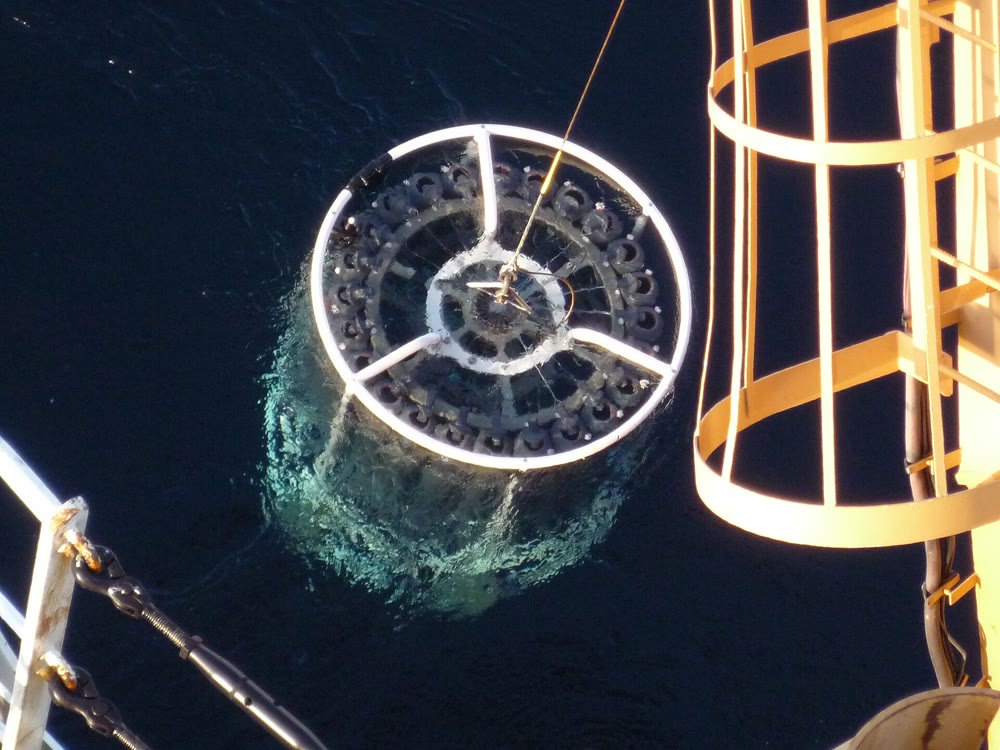
\includegraphics[height=4.4cm]{images/book2/g10-noaa-ctd-rosette.jpg}\hspace{0.4cm}%
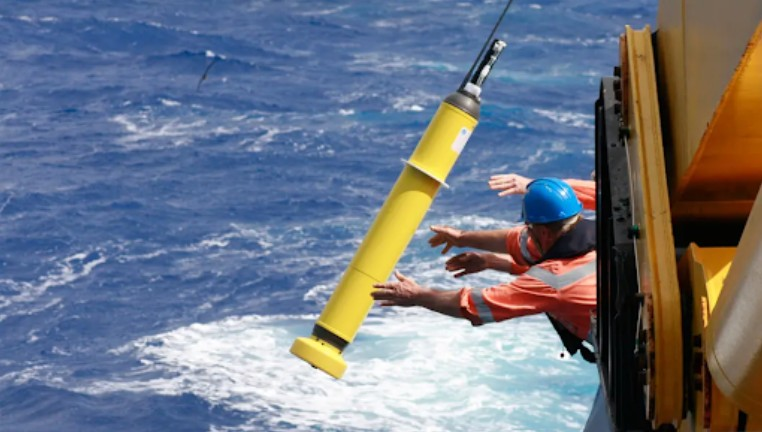
\includegraphics[height=4.4cm]{images/book2/g10-noaa-argo-float.jpg}

{\small À gauche~: une rosette de bouteilles de prélèvement autour de ses
capteurs, remontée le long d'un navire de recherche dans l'Arctique, 2008
(photographie~: Pablo Clemente-Colon, NOAA Photo Library). À droite~: un
flotteur profileur est mis à l'eau depuis un navire de recherche
(photographie~: NOAA Global Ocean Monitoring and Observing Program). Les deux
sont dans le domaine public.}
\end{omfigure}

Moyennés sur des décennies de mesures, ces profils donnent une image de
l'océan en profondeur. Les profils de ce chapitre sont de telles moyennes,
tirées du \emph{World Ocean Atlas 2023} des NOAA National Centers for
Environmental Information.

\section{La température en profondeur}

\begin{omfigure}
\begin{tikzpicture}
\begin{axis}[omrecord, omdepth, width=0.62\linewidth, height=8.2cm,
  axis x line=top, xmin=-3, xmax=31, ymin=0, ymax=2000,
  xlabel={température (\unit{\degreeCelsius})}, ylabel={profondeur (\unit{m})},
  tick label style={font=\small}, label style={font=\small},
  legend style={font=\scriptsize, at={(0.98,0.03)}, anchor=south east}]
\addplot[omThm!85!black, thick] table[x=t, y=depth] {figdata/out/grade-10-ocean_profiles-site-warmpool.dat};
\addplot[omDef!85!black, thick] table[x=t, y=depth] {figdata/out/grade-10-ocean_profiles-site-atlantic.dat};
\addplot[black!70, thick, dashed] table[x=t, y=depth] {figdata/out/grade-10-ocean_profiles-site-arctic.dat};
\legend{{Pacifique tropical, 5.5\textdegree N}, {Atlantique Nord, 40.5\textdegree N}, {océan Arctique, 75.5\textdegree N}}
\node[font=\scriptsize, anchor=west] (ml) at (axis cs:21,430) {couche de mélange};
\draw[black!50] (ml.north east) -- (axis cs:28.9,35);
\node[font=\scriptsize, anchor=west] (tc) at (axis cs:15.5,600) {thermocline};
\draw[black!50] (tc.north) -- (axis cs:19.9,150);
\node[font=\scriptsize, anchor=west] at (axis cs:7,1500) {océan profond};
\end{axis}
\end{tikzpicture}

{\small Température moyenne en fonction de la profondeur en trois sites (la
profondeur augmente vers le bas). Données~: World Ocean Atlas 2023, moyennes
annuelles, NOAA NCEI.}
\end{omfigure}
% ledger: data:b2-woa23 (profiles in figdata/grade-10/ocean_profiles.py)

La lumière solaire chauffe l'océan par le haut, dans sa couche de surface.
Le vent et les vagues brassent cette eau chaude en une couche de température
presque uniforme. En dessous, la température chute vite sur quelques
centaines de mètres~; plus bas encore, elle baisse lentement jusqu'à l'eau
froide qui remplit les bassins océaniques.

\begin{definition}[Couche de mélange]\label{def:g10:layered-ocean:mixed-layer}
La \emph{couche de mélange}\index{couche de melange@couche de mélange} est
la couche de surface de l'océan, brassée par le vent et les vagues, dans
laquelle la température et la salinité varient à peine avec la profondeur.
\end{definition}

\begin{definition}[Thermocline~; halocline~; pycnocline~; océan profond]\label{def:g10:layered-ocean:thermocline}
La \emph{thermocline}\index{thermocline} est la couche située sous la \omterm{def:g10:layered-ocean:mixed-layer}{couche
de mélange}, dans laquelle la température chute vite avec la profondeur. La
couche dans laquelle la salinité change vite avec la profondeur est une
\emph{halocline}\index{halocline}~; la couche dans laquelle la masse
volumique augmente vite avec la profondeur est la
\emph{pycnocline}\index{pycnocline}. En dessous s'étend l'\emph{océan
profond}\index{ocean profond@océan profond}, froid et lentement changeant.
\end{definition}

Dans le Pacifique tropical, la \omterm{def:g10:layered-ocean:mixed-layer}{couche de mélange} est à
\qty{29.2}{\degreeCelsius} et épaisse d'environ \qty{60}{m}~; entre
\qty{70}{m} et \qty{300}{m}, la température baisse de près de dix-neuf
degrés, et à \qty{1000}{m} elle n'est plus que de \qty{4.5}{\degreeCelsius}.
Dans l'Atlantique Nord, la surface est plus fraîche et la baisse plus
progressive. Dans l'océan Arctique, toute la colonne reste à moins de deux
degrés de \qty{0}{\degreeCelsius}~: il n'y a pour ainsi dire pas de couche
de surface chaude.
% ledger: data:b2-woa23

\begin{method}[Lire un profil océanique]\label{met:g10:layered-ocean:profile}
\begin{enumerate}
  \item Repérer les axes~: la profondeur augmente vers le bas, la grandeur
        mesurée se lit en haut.
  \item La \omterm{def:g10:layered-ocean:mixed-layer}{couche de mélange} est la partie haute où la courbe est presque
        verticale~; sa profondeur est celle où la courbe commence à
        s'infléchir (une règle courante~: là où la température a baissé de
        \qty{0.5}{\degreeCelsius} par rapport à sa valeur de surface).
  \item La \omterm{def:g10:layered-ocean:thermocline}{thermocline} est là où la courbe est la plus proche de
        l'horizontale~: le plus grand changement sur la plus petite
        profondeur.
  \item Plus bas, lire les valeurs profondes et comparer les sites à la même
        profondeur.
\end{enumerate}
\end{method}

La \omterm{def:g10:layered-ocean:mixed-layer}{couche de mélange} change avec les saisons. En hiver, la surface perd de
la chaleur, les tempêtes brassent la mer, et la \omterm{def:g10:layered-ocean:mixed-layer}{couche de mélange}
s'approfondit~; en été, le soleil réchauffe une mince couche de surface que
les vents, plus doux, ne peuvent mélanger vers le bas, et une
\emph{\omterm{def:g10:layered-ocean:thermocline}{thermocline} saisonnière} se forme près de la surface --- l'eau froide
que trouvent les pieds du nageur.

\begin{omfigure}
\begin{tikzpicture}
\begin{axis}[omrecord, omdepth, width=0.6\linewidth, height=6.6cm,
  axis x line=top, xmin=12, xmax=24, ymin=0, ymax=300,
  xlabel={température (\unit{\degreeCelsius})}, ylabel={profondeur (\unit{m})},
  tick label style={font=\small}, label style={font=\small},
  legend style={font=\scriptsize, at={(0.98,0.03)}, anchor=south east}]
\addplot[omDef!85!black, thick] table[x=t_feb, y=depth] {figdata/out/grade-10-ocean_profiles-season.dat};
\addplot[omThm!85!black, thick] table[x=t_aug, y=depth] {figdata/out/grade-10-ocean_profiles-season.dat};
\legend{février, août}
\end{axis}
\end{tikzpicture}

{\small L'hiver et l'été dans l'Atlantique Nord (40.5\textdegree N,
30.5\textdegree O)~: températures moyennes mensuelles de février et d'août.
En février, la \omterm{def:g10:layered-ocean:mixed-layer}{couche de mélange} atteint environ \qty{170}{m}~; en août, une
couche chaude d'environ \qty{15}{m} d'épaisseur repose sur une \omterm{def:g10:layered-ocean:thermocline}{thermocline}
saisonnière. Données~: World Ocean Atlas 2023, NOAA NCEI.}
\end{omfigure}
% ledger: data:b2-woa23 (mixed-layer depths by the 0.5 degC rule, computed in figdata/grade-10/ocean_profiles.py)

\section{Salinité et masse volumique}

La masse volumique de l'eau de mer dépend de sa température et de sa
salinité. On la calcule par une formule adoptée au niveau international,
l'équation d'état de l'eau de mer, ajustée sur des mesures de laboratoire.

\begin{proposition}[Masse volumique de l'eau de mer]\label{prop:g10:layered-ocean:density}
La masse volumique de l'eau de mer augmente avec sa salinité et diminue
quand sa température s'élève. À la pression de la surface, une eau de mer de
salinité 35 a une masse volumique de \qty{1028.1}{kg/m^3} à
\qty{0}{\degreeCelsius} et de \qty{1023.3}{kg/m^3} à
\qty{25}{\degreeCelsius}~; l'eau pure à \qty{4}{\degreeCelsius} a une masse
volumique de \qty{1000.0}{kg/m^3}.
\end{proposition}
% ledger: unesco:eos80 (values computed in figdata/grade-10/ocean_profiles.py)

\begin{omfigure}
\begin{tikzpicture}
\begin{axis}[omrecord, width=0.7\linewidth, height=6.2cm, xmin=-2, xmax=30,
  ymin=1016, ymax=1033, xlabel={température (\unit{\degreeCelsius})},
  ylabel={masse volumique (\unit{kg/m^3})}, tick label style={font=\small},
  label style={font=\small}, yticklabel style={/pgf/number format/1000 sep={}}]
\addplot[omThm!85!black, thick] table[x=t, y=rho_s38] {figdata/out/grade-10-ocean_profiles-eos.dat};
\addplot[black!80, thick] table[x=t, y=rho_s35] {figdata/out/grade-10-ocean_profiles-eos.dat};
\addplot[omDef!85!black, thick] table[x=t, y=rho_s30] {figdata/out/grade-10-ocean_profiles-eos.dat};
\node[font=\scriptsize, anchor=south west, omThm!85!black] at (axis cs:1,1030.75) {salinité 38};
\node[font=\scriptsize, anchor=south west] at (axis cs:1,1028.35) {salinité 35};
\node[font=\scriptsize, anchor=south west, omDef!85!black] at (axis cs:1,1024.35) {salinité 30};
\end{axis}
\end{tikzpicture}

{\small La masse volumique de l'eau de mer à la pression de la surface, en
fonction de sa température, pour trois salinités (calculée par l'équation
d'état internationale de l'eau de mer).}
\end{omfigure}
% ledger: unesco:eos80

Le graphique montre deux choses. Une unité de salinité ajoute environ
\qty{0.8}{kg/m^3}. Un degré de réchauffement retire environ
\qty{0.31}{kg/m^3} à \qty{25}{\degreeCelsius}, \qty{0.18}{kg/m^3} à
\qty{10}{\degreeCelsius}, mais seulement \qty{0.06}{kg/m^3} près de
\qty{0}{\degreeCelsius}~: dans les mers chaudes, c'est la température qui
commande la masse volumique, dans les mers froides, c'est la salinité.
% ledger: unesco:eos80 (slopes computed in figdata/grade-10/ocean_profiles.py)

\begin{remark}
Les masses volumiques de ce chapitre sont calculées à la pression de la
surface. La pression de l'eau située au-dessus comprime un peu l'eau de
mer, d'environ \qty{4}{kg/m^3} par kilomètre de profondeur~; les
océanographes comparent les masses d'eau à la même pression, pour que seules
la température et la salinité comptent.
\end{remark}
% ledger: unesco:eos80-checks (computed in figdata/grade-10/ocean_profiles.py: 3.9 kg/m3 per km from the 10000-dbar check values)

\begin{omfigure}
\begin{tikzpicture}
\begin{axis}[name=sal, omrecord, omdepth, width=0.5\linewidth, height=7.2cm,
  axis x line=top, xmin=27.5, xmax=37, ymin=0, ymax=1000,
  xlabel={salinité}, ylabel={profondeur (\unit{m})},
  tick label style={font=\small}, label style={font=\small}]
\addplot[omThm!85!black, thick] table[x=s, y=depth] {figdata/out/grade-10-ocean_profiles-site-warmpool.dat};
\addplot[omDef!85!black, thick] table[x=s, y=depth] {figdata/out/grade-10-ocean_profiles-site-atlantic.dat};
\addplot[black!70, thick, dashed] table[x=s, y=depth] {figdata/out/grade-10-ocean_profiles-site-arctic.dat};
\node[font=\scriptsize, anchor=west, align=left] at (axis cs:28.2,120) {halocline\\arctique};
\end{axis}
\begin{axis}[at={(sal.east)}, anchor=west, xshift=0.9cm, omrecord, omdepth,
  width=0.5\linewidth, height=7.2cm, axis x line=top, xmin=1021, xmax=1028.5, yticklabels={},
  ymin=0, ymax=1000, xlabel={masse volumique (\unit{kg/m^3})},
  tick label style={font=\small}, label style={font=\small},
  xticklabel style={/pgf/number format/1000 sep={}},
  legend style={font=\scriptsize, at={(0.03,0.03)}, anchor=south west}]
\addplot[omThm!85!black, thick] table[x=rho, y=depth] {figdata/out/grade-10-ocean_profiles-site-warmpool.dat};
\addplot[omDef!85!black, thick] table[x=rho, y=depth] {figdata/out/grade-10-ocean_profiles-site-atlantic.dat};
\addplot[black!70, thick, dashed] table[x=rho, y=depth] {figdata/out/grade-10-ocean_profiles-site-arctic.dat};
\legend{Pacifique tropical, Atlantique Nord, océan Arctique}
\end{axis}
\end{tikzpicture}

{\small La salinité (à gauche) et la masse volumique à la pression de la
surface (à droite) en fonction de la profondeur, aux trois sites des profils
de température. Partout, la masse volumique augmente vers le bas.
Données~: World Ocean Atlas 2023, NOAA NCEI~; masses volumiques calculées
par l'équation d'état internationale de l'eau de mer.}
\end{omfigure}
% ledger: data:b2-woa23, unesco:eos80

Dans le Pacifique tropical, la \omterm{def:g10:layered-ocean:thermocline}{pycnocline} coïncide avec la \omterm{def:g10:layered-ocean:thermocline}{thermocline}. Dans
l'océan Arctique, la température change à peine, mais la salinité passe de
28 en surface, adoucie par les fleuves et la fonte des glaces, à 34.8 à
\qty{500}{m}~: la \omterm{def:g10:layered-ocean:thermocline}{halocline} est la \omterm{def:g10:layered-ocean:thermocline}{pycnocline}. Dans chaque cas, la masse
volumique augmente vers le bas.
% ledger: data:b2-woa23

\begin{definition}[Stratification]\label{def:g10:layered-ocean:stratification}
L'océan est \emph{stratifié}\index{stratification} quand sa masse volumique
augmente avec la profondeur~: l'eau plus légère repose sur l'eau plus dense,
en couches.
\end{definition}

Un océan \omterm{def:g10:layered-ocean:stratification}{stratifié} est stable. Une parcelle d'eau poussée vers le bas dans
une eau plus dense est plus légère que son environnement et remonte~; une
parcelle poussée vers le haut redescend. Pour mélanger les couches, le vent
doit lutter contre cet effet, et plus la \omterm{def:g10:layered-ocean:thermocline}{pycnocline} est marquée, plus c'est
difficile~: la \omterm{def:g10:layered-ocean:thermocline}{thermocline} est un couvercle qui sépare la surface de
l'\omterm{def:g10:layered-ocean:thermocline}{océan profond}. L'\omterm{def:g10:layered-ocean:thermocline}{océan profond} est rempli d'une eau qui a plongé il y a
longtemps depuis les mers polaires froides, où l'eau de surface devient
assez dense pour couler (livre~1, année~8).

\section{Les remontées d'eau}

\begin{definition}[Remontée d'eau]\label{def:g10:layered-ocean:upwelling}
Une \emph{remontée d'eau}\index{remontee d'eau@remontée d'eau} (on dit aussi
«~upwelling~») est la montée d'eau froide venue de sous la couche de
surface, pour remplacer l'eau de surface que le vent repousse. Elle se
produit le long de certaines côtes et en plein océan.
\end{definition}
% ledger: noaa:upwelling

Le long d'une côte, le vent qui souffle parallèlement au rivage entraîne
l'eau de surface~; à cause de la rotation de la Terre, l'eau ne suit pas
simplement le vent mais en est déviée, vers la droite dans l'hémisphère Nord
et vers la gauche dans l'hémisphère Sud (le mécanisme est l'objet des
volumes universitaires). Au large du Pérou, le vent souffle le long du
rivage vers l'équateur, et l'eau de surface est repoussée vers le large~;
de l'eau froide remonte près de la côte pour prendre sa place. Des \omterm{def:g10:layered-ocean:upwelling}{remontées
d'eau} se produisent aussi le long de l'équateur, où les alizés écartent
l'eau de surface de part et d'autre.
% ledger: noaa:upwelling, kessler:peru-upwelling

\begin{omfigure}
\begin{tikzpicture}[font=\footnotesize, >={Stealth[length=2mm]}]
  % ocean and thermocline
  \fill[omDef!12] (0,-3.2) rectangle (8.2,0);
  \fill[omDef!30] (0,-3.2) -- (0,-2.0) .. controls (3,-2.0) and (5.5,-1.6) .. (7.4,-0.35) -- (8.2,0) -- (8.2,-3.2) -- cycle;
  \draw[omDef!80!black, dashed] (0,-2.0) .. controls (3,-2.0) and (5.5,-1.6) .. (7.4,-0.35);
  \node[anchor=north west, omDef!80!black] at (0.1,-2.05) {thermocline};
  \node[anchor=west, black!70] at (0.15,-0.9) {eau de surface chaude};
  \node[anchor=west, black!70] at (0.15,-2.75) {eau froide, riche en nutriments};
  % land
  \fill[omExo!30, draw=black!60] (7.0,-3.2) -- (8.2,-0.1) -- (8.6,0.0) -- (9.6,1.2) -- (10.6,2.2) -- (10.6,-3.2) -- cycle;
  \node[anchor=south, align=center] at (9.9,-1.6) {terre};
  % surface flow and rising water
  \draw[->, thick, omThm!80!black] (7.2,-0.3) -- (3.6,-0.3);
  \node[anchor=south, omThm!80!black] at (5.4,-0.25) {eau de surface repoussée vers le large};
  \foreach \x/\y in {6.1/-2.1, 6.8/-1.7} \draw[->, thick, omDef!80!black] (\x,\y) -- (\x+0.45,\y+1.15);
  \node[anchor=north, omDef!80!black, align=center] at (6.0,-2.25) {l'eau froide remonte};
  % wind along the shore, northward: with west on the left and east on the
  % right the reader looks north, so the wind goes into the page
  \draw[black!70, thick] (2.6,1.0) circle (0.22);
  \draw[black!70, thick] (2.6,1.0) ++(45:0.22) -- ++(225:0.44) (2.6,1.0) ++(135:0.22) -- ++(315:0.44);
  \node[anchor=west, align=left] at (2.9,1.0) {vent le long du rivage, vers l'équateur\\(vers le nord, entrant dans la page)};
  \node[anchor=north west, black!60] at (0,-3.25) {$\leftarrow$ ouest};
  \node[anchor=north east, black!60] at (10.6,-3.25) {est $\rightarrow$};
\end{tikzpicture}

{\small \omterm{def:g10:layered-ocean:upwelling}{Remontée d'eau} côtière au large du Pérou (coupe schématique d'ouest
en est, sans échelle)~: le vent souffle le long du rivage vers l'équateur,
vers le nord, en entrant dans la page~; l'eau de surface est déviée vers sa
gauche et repoussée vers le large~; de l'eau froide venue de sous la
\omterm{def:g10:layered-ocean:thermocline}{thermocline} remonte près de la côte pour la remplacer.}
\end{omfigure}

L'eau qui remonte n'est pas seulement froide. Sous la couche de surface
éclairée, les restes de plancton mort qui coulent et se décomposent
libèrent les sels minéraux nutritifs dont le phytoplancton a besoin.
Ramenés à la lumière, ces nutriments font des régions de \omterm{def:g10:layered-ocean:upwelling}{remontée d'eau} les
eaux les plus productives de l'océan, avec les zones de pêche les plus
riches. Là où l'océan est fortement \omterm{def:g10:layered-ocean:stratification}{stratifié} et où rien ne fait remonter
l'eau profonde, la couche éclairée s'épuise en nutriments~: le centre des
gyres subtropicaux est le désert de l'océan.
% ledger: noaa:upwelling

\begin{omfigure}
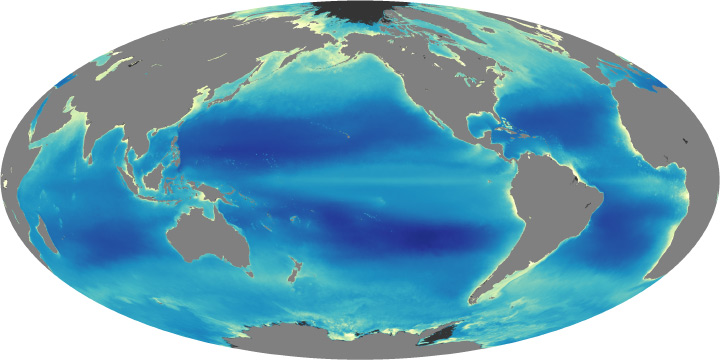
\includegraphics[width=0.8\linewidth]{images/book2/g10-nasa-ocean-chlorophyll.jpg}

{\small La chlorophylle du phytoplancton vue de l'espace, en moyenne sur
2002--2010~: du bleu foncé (très peu) au bleu clair puis au jaune
(beaucoup)~; les terres en gris. La côte du Pérou et la bande qui longe
l'équateur dans le Pacifique ressortent~; les gyres sont d'un bleu profond.
Image~: Jesse Allen et Robert Simmon, NASA Earth Observatory (domaine
public).}
\end{omfigure}

\begin{omfigure}
\begin{tikzpicture}
\begin{axis}[omrecord, omdepth, width=0.6\linewidth, height=7.2cm,
  axis x line=top, xmin=4, xmax=26, ymin=0, ymax=600,
  xlabel={température (\unit{\degreeCelsius})}, ylabel={profondeur (\unit{m})},
  tick label style={font=\small}, label style={font=\small},
  legend style={font=\scriptsize, at={(0.98,0.03)}, anchor=south east}]
\addplot[omExo!85!black, thick] table[x=t, y=depth] {figdata/out/grade-10-ocean_profiles-site-peru.dat};
\addplot[omThm!85!black, thick] table[x=t, y=depth] {figdata/out/grade-10-ocean_profiles-site-gyre.dat};
\addplot[black!40, dashed, domain=0:600, samples=2] ({15}, {x});
\legend{{au large du Pérou, 13.5\textdegree S}, {gyre du Pacifique Sud, 20.5\textdegree S}}
\end{axis}
\end{tikzpicture}

{\small Au large du Pérou, l'eau froide s'approche de la surface~: l'eau à
\qty{15}{\degreeCelsius} (tirets) se trouve vers \qty{65}{m}, contre près de
\qty{300}{m} au milieu du gyre du Pacifique Sud, plus éloigné de l'équateur.
Données~: World Ocean Atlas 2023, moyennes annuelles, NOAA NCEI.}
\end{omfigure}
% ledger: data:b2-woa23

\section{Exercices}

\begin{exercise}[$\star$]\label{exo:g10:layered-ocean:1}
Définir la \omterm{def:g10:layered-ocean:mixed-layer}{couche de mélange} et la \omterm{def:g10:layered-ocean:thermocline}{thermocline}. Qu'est-ce qui brasse la
\omterm{def:g10:layered-ocean:mixed-layer}{couche de mélange}~?
\end{exercise}

\begin{exercise}[$\star$]\label{exo:g10:layered-ocean:2}
Définir une \omterm{def:g10:layered-ocean:upwelling}{remontée d'eau}. Pourquoi les eaux des régions de \omterm{def:g10:layered-ocean:upwelling}{remontée d'eau}
sont-elles riches en vie~?
\end{exercise}

\begin{exercise}[$\star$]\label{exo:g10:layered-ocean:3}
À l'aide des profils de température des trois sites, donner la température
en surface et à \qty{1000}{m} dans le Pacifique tropical et dans l'océan
Arctique.
\end{exercise}

\begin{exercise}[$\star$]\label{exo:g10:layered-ocean:4}
Laquelle est la plus dense, une eau de mer de salinité 35 à
\qty{25}{\degreeCelsius} ou à \qty{0}{\degreeCelsius}~? Une eau de mer de
salinité 35 ou de l'eau pure, à la même température~? Utiliser les valeurs
du chapitre.
\end{exercise}

\begin{exercise}[$\star$]\label{exo:g10:layered-ocean:5}
Expliquer comment un flotteur profileur mesure un profil de l'océan, et
pourquoi les flotteurs sont utiles là où les navires vont rarement.
\end{exercise}

\begin{exercise}[$\star\star$]\label{exo:g10:layered-ocean:6}
L'océan couvre \num{361.84}~millions de~\unit{km^2} avec une profondeur
moyenne de \qty{3682}{m}. Calculer son volume en kilomètres cubes. Quelle
fraction de sa profondeur représentent les \qty{100}{m} supérieurs~?
\end{exercise}

\begin{exercise}[$\star\star$]\label{exo:g10:layered-ocean:7}
Dans le profil d'août de l'Atlantique Nord, la température vaut
\qty{22.7}{\degreeCelsius} en surface, \qty{22.2}{\degreeCelsius} à
\qty{15}{m}, \qty{21.8}{\degreeCelsius} à \qty{20}{m} et
\qty{17.3}{\degreeCelsius} à \qty{50}{m}. À l'aide de la règle de la
méthode, estimer la profondeur de la \omterm{def:g10:layered-ocean:mixed-layer}{couche de mélange}. Quel est le rythme
moyen de baisse de la température entre \qty{20}{m} et \qty{50}{m}, en
degrés par mètre~?
\end{exercise}

\begin{exercise}[$\star\star$]\label{exo:g10:layered-ocean:8}
Au même site de l'Atlantique Nord, la surface est à
\qty{15.3}{\degreeCelsius} en février et à \qty{22.7}{\degreeCelsius} en
août, tandis qu'à \qty{300}{m} elle est à \qty{13.5}{\degreeCelsius} les
deux mois. Expliquer pourquoi l'eau profonde ne suit pas les saisons, et
pourquoi la \omterm{def:g10:layered-ocean:mixed-layer}{couche de mélange} d'hiver est bien plus profonde que celle
d'été.
\end{exercise}

\begin{exercise}[$\star\star$]\label{exo:g10:layered-ocean:9}
Vers \qty{10}{\degreeCelsius}, une unité de salinité ajoute
\qty{0.78}{kg/m^3} à la masse volumique et un degré de réchauffement en
retire \qty{0.18}{kg/m^3}. Combien de degrés de réchauffement compensent une
unité de salinité~? Répondre à la même question vers
\qty{0}{\degreeCelsius}, où un degré ne retire que \qty{0.06}{kg/m^3}. Que
peut-on en conclure pour les mers polaires~?
\end{exercise}

\begin{exercise}[$\star\star$]\label{exo:g10:layered-ocean:10}
Dans l'océan Arctique, l'eau de surface est à \qty{-1.4}{\degreeCelsius}
avec une salinité de 28.1, et l'eau à \qty{200}{m} à
\qty{-1.4}{\degreeCelsius} avec une salinité de 33.3. Leurs masses
volumiques sont \qty{1022.6}{kg/m^3} et \qty{1026.8}{kg/m^3}. Qu'est-ce qui
rend l'eau profonde plus dense~? Nommer la couche qui les sépare.
\end{exercise}

\begin{exercise}[$\star\star$]\label{exo:g10:layered-ocean:11}
Expliquer pourquoi un océan \omterm{def:g10:layered-ocean:stratification}{stratifié} est stable, à l'aide d'une parcelle
d'eau de surface poussée vers le bas par une vague.
\end{exercise}

\begin{exercise}[$\star\star\star$]\label{exo:g10:layered-ocean:12}
Un litre d'eau de mer de salinité 35 à \qty{0}{\degreeCelsius} est chauffé
à \qty{25}{\degreeCelsius}. À l'aide des masses volumiques du chapitre,
calculer sa masse, puis son nouveau volume. De combien s'est-il dilaté, en
millilitres~? Une couche d'océan de \qty{700}{m} d'épaisseur se réchauffe
dans la même proportion~: de combien son épaisseur augmente-t-elle~? (C'est
une forte exagération du réchauffement réel de l'océan, utilisée ici
seulement pour montrer l'effet.)
\end{exercise}

\begin{exercise}[$\star\star\star$]\label{exo:g10:layered-ocean:13}
Dans le Pacifique tropical, la masse volumique vaut \qty{1021.6}{kg/m^3} à
\qty{50}{m} et \qty{1026.0}{kg/m^3} à \qty{200}{m}~; dans l'Atlantique Nord
en février, la température change à peine sur les \qty{150}{m} supérieurs.
Dans lequel des deux une tempête aurait-elle le plus de facilité à brasser
l'eau jusqu'à \qty{150}{m}~? Expliquer.
\end{exercise}

\begin{exercise}[$\star\star\star$]\label{exo:g10:layered-ocean:14}
Sur la carte de la chlorophylle, trouver deux régions riches en
chlorophylle en plein océan, loin de toute côte, et une vaste région très
pauvre en chlorophylle. À l'aide du chapitre, expliquer chacune.
\end{exercise}

\begin{exercise}[$\star\star\star$]\label{exo:g10:layered-ocean:15}
On suppose qu'un flotteur plonge de \qty{1000}{m} à \qty{2000}{m} en six
heures, puis remonte à la surface en dix heures. Calculer sa vitesse
verticale moyenne dans chaque phase, en centimètres par seconde. S'il fait
une mesure toutes les \qty{2}{s} pendant la remontée, combien de mesures un
profil contient-il, et quelle profondeur en sépare deux en moyenne~?
\end{exercise}

\section{Problème~: une station au large du Pérou}

\begin{problem}[{Problème du week-end --- deux profils du Pacifique Sud}]
\label{pb:g10:layered-ocean:1}
% ledger: data:b2-woa23, unesco:eos80 (values rounded from figdata/grade-10/ocean_profiles.py)
Le tableau donne la température et la salinité moyennes, ainsi que la masse
volumique calculée à la pression de la surface, en deux lieux du Pacifique
Sud~: au large du Pérou (\qty{13.5}{\degree S}, \qty{77.5}{\degree O}) et au
milieu du gyre subtropical (\qty{20.5}{\degree S}, \qty{110.5}{\degree O}).

\begin{center}
\small
\begin{tabular}{c|ccc|ccc}
\hline
 & \multicolumn{3}{c|}{au large du Pérou} & \multicolumn{3}{c}{gyre} \\
profondeur (\unit{m}) & \unit{\degreeCelsius} & salinité & \unit{kg/m^3} & \unit{\degreeCelsius} & salinité & \unit{kg/m^3} \\
\hline
0 & 19.0 & 35.08 & 1025.08 & 24.0 & 36.41 & 1024.71 \\
25 & 17.4 & 35.06 & 1025.47 & 23.9 & 36.39 & 1024.73 \\
50 & 15.8 & 35.03 & 1025.83 & 23.6 & 36.38 & 1024.80 \\
100 & 13.7 & 34.93 & 1026.20 & 22.6 & 36.27 & 1025.02 \\
200 & 12.4 & 34.89 & 1026.44 & 20.3 & 35.80 & 1025.30 \\
300 & 11.1 & 34.80 & 1026.62 & 14.4 & 34.76 & 1025.92 \\
500 & 7.9 & 34.60 & 1026.97 & 7.1 & 34.39 & 1026.92 \\
\hline
\end{tabular}
\end{center}

\medskip
\noindent\textbf{Partie I --- Lire les profils.}
\begin{enumerate}
  \item Quel site est le plus chaud en surface, et de combien~?
  \item Quel site est le plus éloigné de l'équateur~? L'écart de
        température de surface est-il celui qu'on attendrait des seules
        latitudes~?
  \item À l'aide de la règle de la méthode, estimer la profondeur de la
        \omterm{def:g10:layered-ocean:mixed-layer}{couche de mélange} dans le gyre.
  \item Y a-t-il une \omterm{def:g10:layered-ocean:mixed-layer}{couche de mélange} au large du Pérou~? Décrire les
        \qty{100}{m} supérieurs.
  \item Entre quelles profondeurs la température baisse-t-elle le plus vite
        dans le gyre~? Donner le rythme, en degrés par centaine de mètres.
  \item À quelle profondeur, à peu près, se trouve l'eau à
        \qty{15}{\degreeCelsius} sur chaque site~?
\end{enumerate}

\medskip
\noindent\textbf{Partie II --- Les masses volumiques.}
\begin{enumerate}[resume]
  \item Vérifier que la masse volumique augmente avec la profondeur sur les
        deux sites. Qu'est-ce que cela indique sur leur stabilité~?
  \item Dans le gyre, l'eau de surface est plus salée qu'au large du Pérou.
        Cela devrait-il la rendre plus dense ou plus légère~? Est-elle plus
        dense~?
  \item Expliquer lequel des deux effets l'emporte.
  \item Calculer l'augmentation de la masse volumique de la surface à
        \qty{200}{m} au large du Pérou.
  \item Calculer la même augmentation dans le gyre.
\end{enumerate}

\medskip
\noindent\textbf{Partie III --- Deux stratifications comparées.}
\begin{enumerate}[resume]
  \item Dans le gyre, où se trouve l'essentiel de l'augmentation de masse
        volumique des \qty{500}{m} supérieurs~: au-dessus ou en dessous de
        \qty{200}{m}~?
  \item Au large du Pérou, où se trouve-t-il~?
  \item À \qty{500}{m}, comparer les deux sites. Que cela suggère-t-il sur
        l'eau profonde située sous les deux~?
  \item Expliquer en quelques phrases comment la \omterm{def:g10:layered-ocean:thermocline}{thermocline} a été soulevée
        vers la surface au large du Pérou.
  \item Le phytoplancton vit dans les quelques dizaines de mètres
        supérieurs. Sur quel site l'eau riche en nutriments venue de sous la
        \omterm{def:g10:layered-ocean:thermocline}{thermocline} est-elle à portée du brassage par le vent~? Expliquer.
\end{enumerate}

\medskip
\noindent\textbf{Partie IV --- Pourquoi les eaux péruviennes sont productives.}
\begin{enumerate}[resume]
  \item À quoi ressemblerait l'eau de surface au large du Pérou si le vent
        cessait de souffler le long du rivage pendant des mois~?
  \item À l'aide de la carte de la chlorophylle, comparer les deux sites.
  \item Expliquer pourquoi le gyre est appelé un désert de l'océan bien
        qu'il soit inondé de lumière solaire.
  \item Calculer le rapport des augmentations de masse volumique de la
        surface à \qty{200}{m} au large du Pérou et dans le gyre, et dire ce
        qu'il montre.
\end{enumerate}
\end{problem}
